\part{Ejercicio 3}
\section{Enunciado}
Dado un arreglo de $n$ elementos en el que hay un elemento que aparece m'as de la mitad de las 
veces, encontrar la moda, es decir, el valor que aparece m'as veces.

\section{Desarrollo}
\paragraph{}
La primera idea para abordar este problema fue la de ordenar el arreglo y contar la cantidad 
de apariciones guardando el elemento con m'as apariciones. Esta primera idea no tuvo mucha 
aceptaci'on ya que se observ'o que el orden requerido para ordenar dicho arreglo no cumpl'ia
con el requisito de ser mejor que $O(n log n)$.
\paragraph{}
Una mejora a este procedimiento fue notar que la moda en un arreglo con las caracter'isticas
dadas por el problema coincide con el elemento $n/2$ del arreglo ordenado (la mediana). Por lo tanto, 
si se ordena el arreglo, en vez de contar apariciones basta con tomar el elemento $n/2$ para 
obtener la moda. Sin embargo, esta mejora tambi'en requiere que el arreglo sea ordenado, y por
lo tanto, al igual que la idea anterior, qued'o descartado por tener un orden de complejidad
demasiado alto.
\paragraph{}
Investigando sobre el tema se encontr'o el algoritmo de Loyd-Pratt-Rivest-Tarjan, que permite 
encontrar la mediana de un arreglo en orden lineal sin necesidad de ordenarlo. El algoritmo 
se basa en el uso de un pivote para partir el arreglo y quedarse solo con la parte donde se 
puede encontrar la mediana. Es necesario para tener orden lineal poder encontrar un buen pivote 
en un orden a lo sumo lineal. El algoritmo resuelve esto partiendo el arreglo principal en arreglos
de 5 elementos, tomando la mediana de 'estos y luego tomando una seudomediana a partir de dicha ``mediana''. 
Se puede demostrar que este procedimiento permite encontrar la mediana en un orden lineal. Esta 
soluci'on se descarto ya que su implementaci'on era bastante complicada, lo cual no resultaba conveniente 
teniendo en cuenta que luego deber'iamos realizar un an'alisis del algoritmo para determinar su
complejidad.
\paragraph{}
Se busc'o entonces otra forma de  obtener un orden lineal aprovechando que la frecuencia de la moda 
era mayor a la mitad. La idea definitiva consiste b'asicamente en recorrer el  arreglo sirvi'endose de 
dos 'indices. Si se encuentran dos elementos iguales, se incrementa uno de los 'indices (en adelante $j$) 
y se deja inm'ovil al otro (en adelante $i$) en la posici'on donde se encuentra. Si se encuentran 2 
elementos diferentes, estos son tachados (para esto se utiliza una marca sobre un arreglo de posiciones booleanas). 
Luego se avanza $i$ hasta que llegue a una posici'on sin tachar y se hace lo propio con $j$ hasta llegar 
a una posici'on sin tachar pero que tambi'en sea mayor que $i$. El ciclo termina cuando $j$ excede el l'imite 
del arreglo. Se devuelve entonces el valor donde qued'o parado el 'indice $i$. 
En cada paso el algoritmo ``tacha'' dos elementos que no son la moda, o uno que es la moda y otro que no. 
De esta forma solo terminan sobreviviendo algunos elementos de la moda. Al terminar el ciclo, los elementos
sin tachar desde $i$ hasta el final del arreglo son iguales. Entonces podr'ian o bien ser moda o ser elementos 
distintos a la moda. Sin embargo, esto 'ultimo no puede ocurrir ya que la frecuencia de la moda es como m'inimo 
$n/2+1$, entonces que eso ocurra implicar'ia que tach'e por lo menos $2*(n/2+1) > n$. Este algoritmo 
fue finalmente el que se adopt'o como soluci'on ya que nos garantizaba el orden lineal buscado y su implementaci'on 
era simple.

\section{Seudoc'odigo}
\newpage
\begin{algorithm}
\caption{Halla la moda $moda$ del arreglo $a$}
\begin{algorithmic}[1]
\STATE indiceDeAtras $\textcolor{orange}{\leftarrow}$ 0
\STATE indiceDeAdelante $\textcolor{orange}{\leftarrow}$ 0
\STATE tachados: [bool] \COMMENT{los elementos de tachados inicializan en false}\\

\WHILE{indiceDeAdelante $\textcolor{orange}{<}$ tamanio\textcolor{magenta}{(}a\textcolor{magenta}{)}}
    \IF{$a_{indiceDeAtras}$ $\textcolor{orange}{\neq}$ $a_{indiceDeAdelante}$}
        \STATE tachados $\textcolor{orange}{\leftarrow}$ tachar ambos elementos //donde: tachar i es asignar con true en el elemento iesimo de tachados
        \WHILE{\textcolor{magenta}{(}indiceDeAtras $\textcolor{orange}{<}$ tamanio\textcolor{magenta}{(}a\textcolor{magenta}{)} \textcolor{orange}{\&} \textcolor{magenta}{(}indiceDeAtras no fue tachado\textcolor{magenta}{)}}
            \STATE indiceDeAtras $\textcolor{orange}{\leftarrow}$ indiceDeAtras \textcolor{orange}{+} 1
        \ENDWHILE
        \WHILE{indiceDeAdelante $\textcolor{orange}{<}$ tamanio\textcolor{magenta}{(}a\textcolor{magenta}{)} \textcolor{orange}{\&} \textcolor{magenta}{(}indiceDeAdelante no fue tachado $\textcolor{orange}{|}$ indiceDeAdelante $\leq$ indiceDeAtras\textcolor{magenta}{)}}
            \STATE indiceDeAdelante $\textcolor{orange}{\leftarrow}$ indiceDeAdelante \textcolor{orange}{+} 1
        \ENDWHILE
    \ELSE
        \STATE indiceDeAdelante $\textcolor{orange}{\leftarrow}$ indiceDeAdelante \textcolor{orange}{+} 1
    \ENDIF

\ENDWHILE
\STATE $moda \textcolor{orange}{\leftarrow}$ $a_{indiceDeAtras}$
\end{algorithmic}
\end{algorithm}


%TODO calculo, demostracion, tamaño de entrada, porq uniforme, peor caso, mejor caso
\section{C'alculo de complejidad}

\section{An'alisis Experimental}
\subsection{Experiencias realizadas}
Nuevamente para este algoritmo se decidi'o medir tanto la cantidad de operaciones como el tiempo en funci'on de la cantidad de 
elementos del arreglo, con la intenci'on de confirmar nuestro analisis te'orico. Para ello se generaron arreglos de largo creciente 
con elementos al azar (distribuci'on uniforme) respetando que la frecuencia de la moda sea de por lo menos $n/2+1$.

Por otro lado para observar la influencia de la frecuencia de la moda en el comportamiento del algoritmo se hicieron corridas de prueba
para un $n$ fijo aumentando la frecuencia y midiendo la cantidad de operaciones y el tiempo insumido.
Adem'as, en algunos casos fue posible utilizar la t'ecnica de cuadrados m'inimos para dar una funci'on 
que aproxime el comportamiento observado experimentalmente. En dichos casos, la ecuaci'on de $f(x)$ se encuentra en el gr'afico.

\subsection{Gr'aficos}

%TODO: rehacer estos graficos es al pedo tener 10^-5 segundos, pasar a milisegundos por lo menos (opcional por ahora)
\begin{figure}[H]
\centering
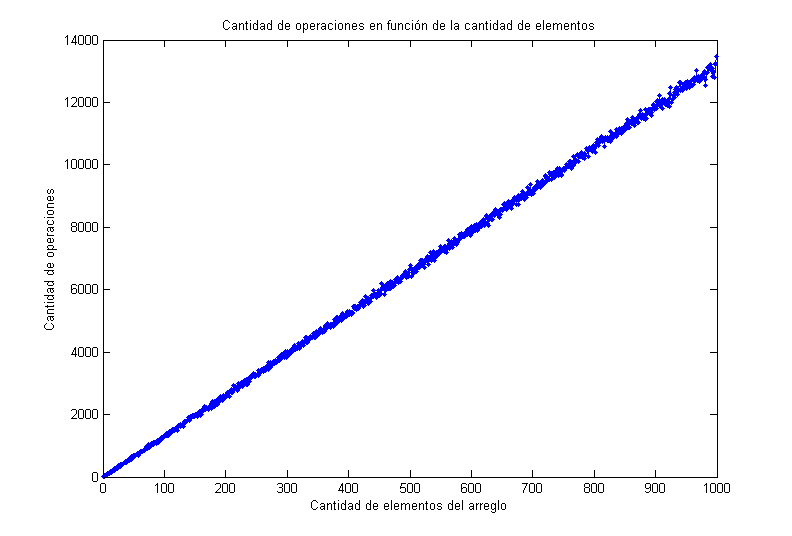
\includegraphics[scale=0.8]{../../codigo/ejercicio3/benchmark/graficos/corridas_aleatorias_n_creciente/grafico.png}
\caption{Cantidad de operaciones en funci'on del tama\~{n}o del arreglo}
\end{figure}

\begin{figure}[H]
\centering
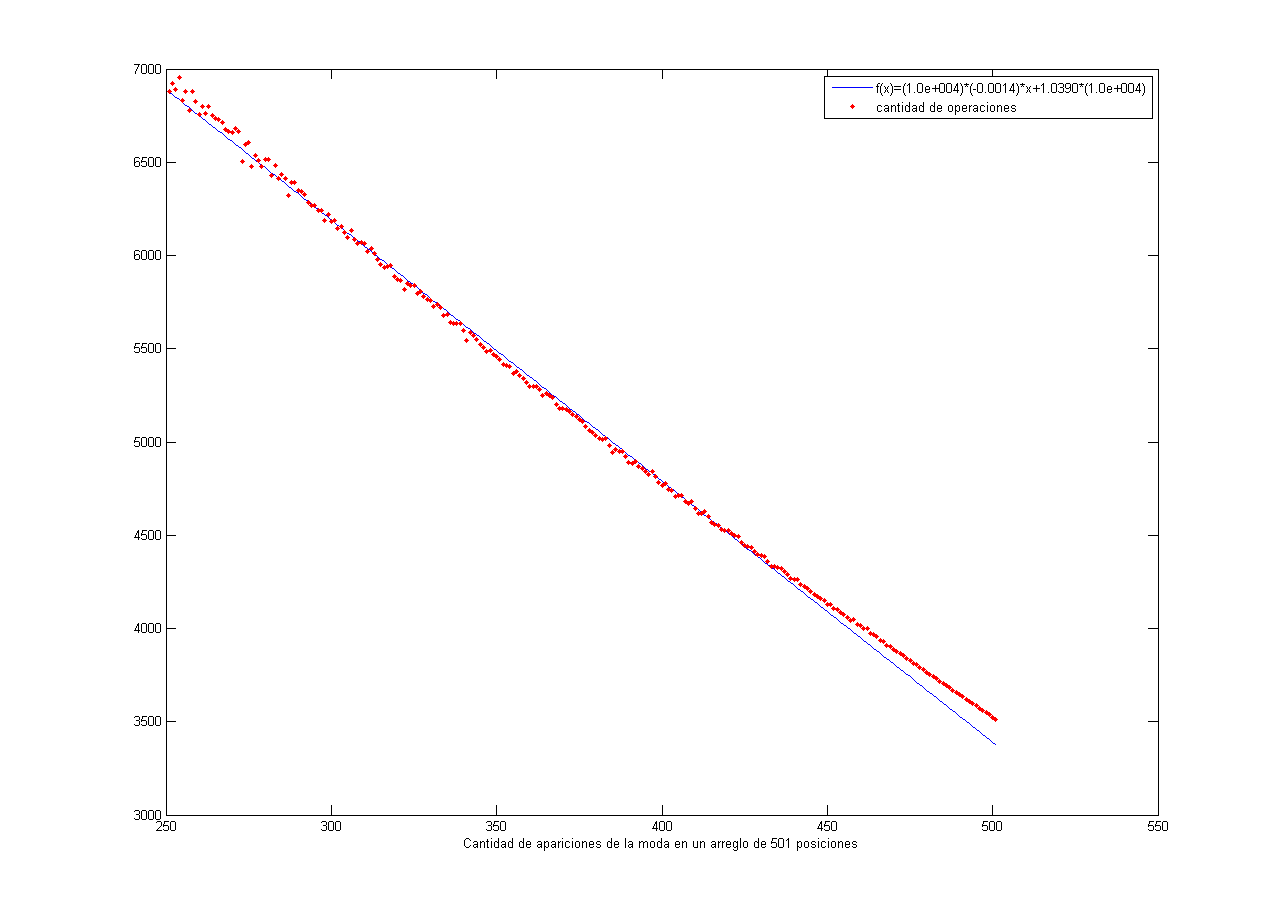
\includegraphics[scale=0.8]{../../codigo/ejercicio3/benchmark/graficos/frecuencia/frecuencia.png}
\caption{Cantidad de operaciones en funci'on de la frecuencia ($n$ = 500)}
\end{figure}

%TODO: rehacer este grafico es al pedo tener 10^-5 segundos, pasar a milisegundos por lo menos 
\begin{figure}[H]
\centering
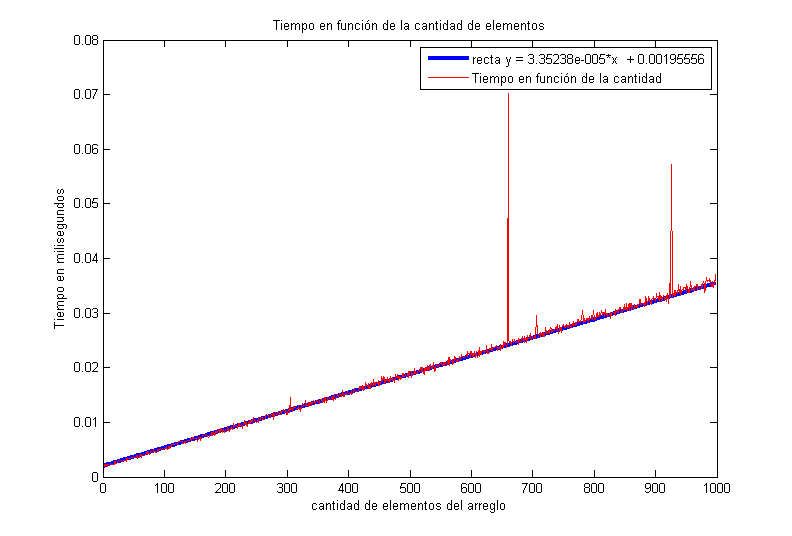
\includegraphics[scale=0.8]{../../codigo/ejercicio3/benchmark_de_tiempo/graficos/moda-1000-casos.png}
\caption{Tiempo (milisegundos) en funci'on del tama\~{n}o del arreglo}
\end{figure}

\begin{figure}[H]
\centering
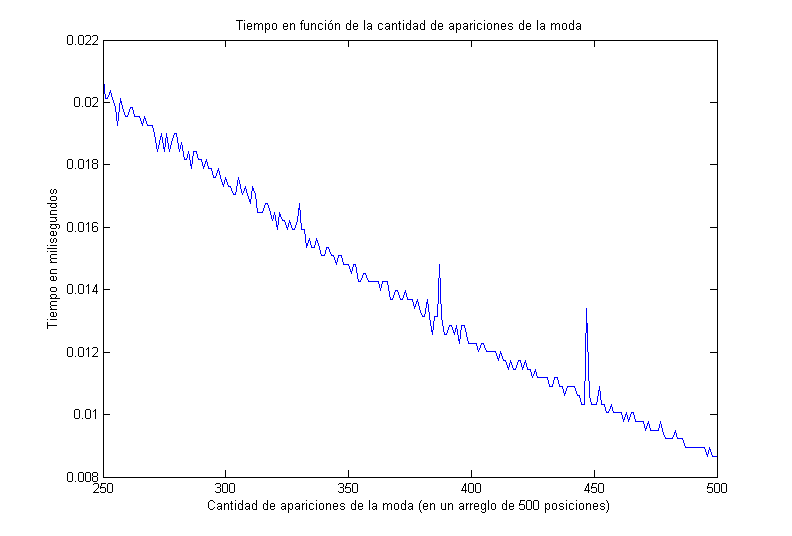
\includegraphics[scale=0.8]{../../codigo/ejercicio3/benchmark_de_tiempo/graficos/aumento-frecuencia.png}
\caption{Tiempo (milisegundos) en funci'on de la frecuencia ($n$ = 500)}
\end{figure}

\section{Discusi'on}
\paragraph{}
En los gr'aficos de tiempo se observ'o que al aumentar el tama\~{n}o del arreglo, el tiempo 
aumenta de forma lineal. Lo mismo ocurre con la cantidad de operaciones. Esta situaci'on se 
corresponde con el an'alisis te'orico que se realiz'o. Por otro lado en los gr'aficos en funci'on 
de la frecuencia de la moda, el tiempo y las operaciones parecieran decrecer linealmente. Esto 
evidencia que el mejor caso se produce cuando todos los elementos del arreglo resultan ser la moda. Esto se
explica de la siguiente manera: si todos los elementos son iguales a la moda, el if de la linea 5 del seudoc'odigo
siempre tiene una condici'on de entrada falsa, por lo que el ciclo recorre el arreglo sin hacer otro tipo de operación.
